% -*- coding: UTF-8 -*-
% vim: autoindent expandtab tabstop=4 sw=4 sts=4 filetype=tex
% vim: spelllang=de spell
% chktex-file 27 - disable warning about missing include files

\section{Vorgehen}
\label{sec:prototype:procedure}

Die Entwicklung des Prototypen war ein iterativer Prozess. Es wurden Teil-Ziele
definiert, welche dann etappenweise erarbeitet wurden.

Das erste Teil-Ziel war das Neu-Kompilieren von Shadern während der Laufzeit,
so dass Shader während der Laufzeit erweitert, neu geladen und dargestellt
werden können.

Als zweites Teil-Ziel wurde dynamisches Laden von Shader-Dateien ausgehend vom
Verzeichnis des Prototypen implementiert.

Als drittes Teil-Ziel wurden Shader in Form von Templates umgesetzt. Mit
``Jinja2CppLight''~\footnote{\href{https://github.com/hughperkins/Jinja2CppLight}{https://github.com/hughperkins/Jinja2CppLight}}
wurde schliesslich ein Template-System eingeführt, welches es erlaubt Shader
als Templates zu parsen und Sektionen entsprechend mit Sub-Templates respektive
Teil-Shadern zu ersetzen.  Dies ermöglicht es Teile von Shadern während der
Laufzeit anzupassen. Durch die Erkenntnisse des ersten Teil-Zieles konnte der
aus dem Template zusammen mit den Sub-Templates generierte Shader zur Laufzeit
geladen und ausgeführt werden.

Als viertes und letztes Teil-Ziel wurde ein Prototyp der Graph-Komponente
(siehe~\autoref{ssubsec:main-components:editor:graph}) umgesetzt. Der Graph bietet
ein Kontext-Menü zum Hinzufügen und Entfernen von Knoten. Für jeden
eingelesenen Teil-Shader wird ein Eintrag im Kontext-Menü hinzugefügt, so dass
dieser schliesslich dem Graphen hinzugefügt werden kann. Der Graph verfügt
standardmässig immer über einen (Haupt-) Ausgangs-Knoten.

Jeder der Knoten verfügt entweder über mindestens einen Eingang oder über einen
Ausgang.  Zusätzliche Ein- beziehungsweise Ausgänge werden je nach Typ eines
Knotens automatisch, dynamisch erstellt. Die Eingänge des Haupt-Knotens sind
jedoch statisch. Dieser verfügt über eine Haupt-Schnittstelle sowie eine
Schnittstelle für einen Kamera-Knoten.

Bei jeder neuen Verbindung beziehungsweise bei jedem Trennen einer Verbindung
innerhalb des Graphen, wird dieser neu evaluiert und die (Shader-) Ausgabe neu
berechnet.

Das Rendering ist schliesslich die Berechnung der relevanten Matrizen, binden
des Shaders und setzen der benötigten Uniform-Variablen.
Abbildung~\ref{fig:prototype:procedure} zeigt den aktuellen Stand des
Prototypen.

\begin{figure}[H]
    \centering
    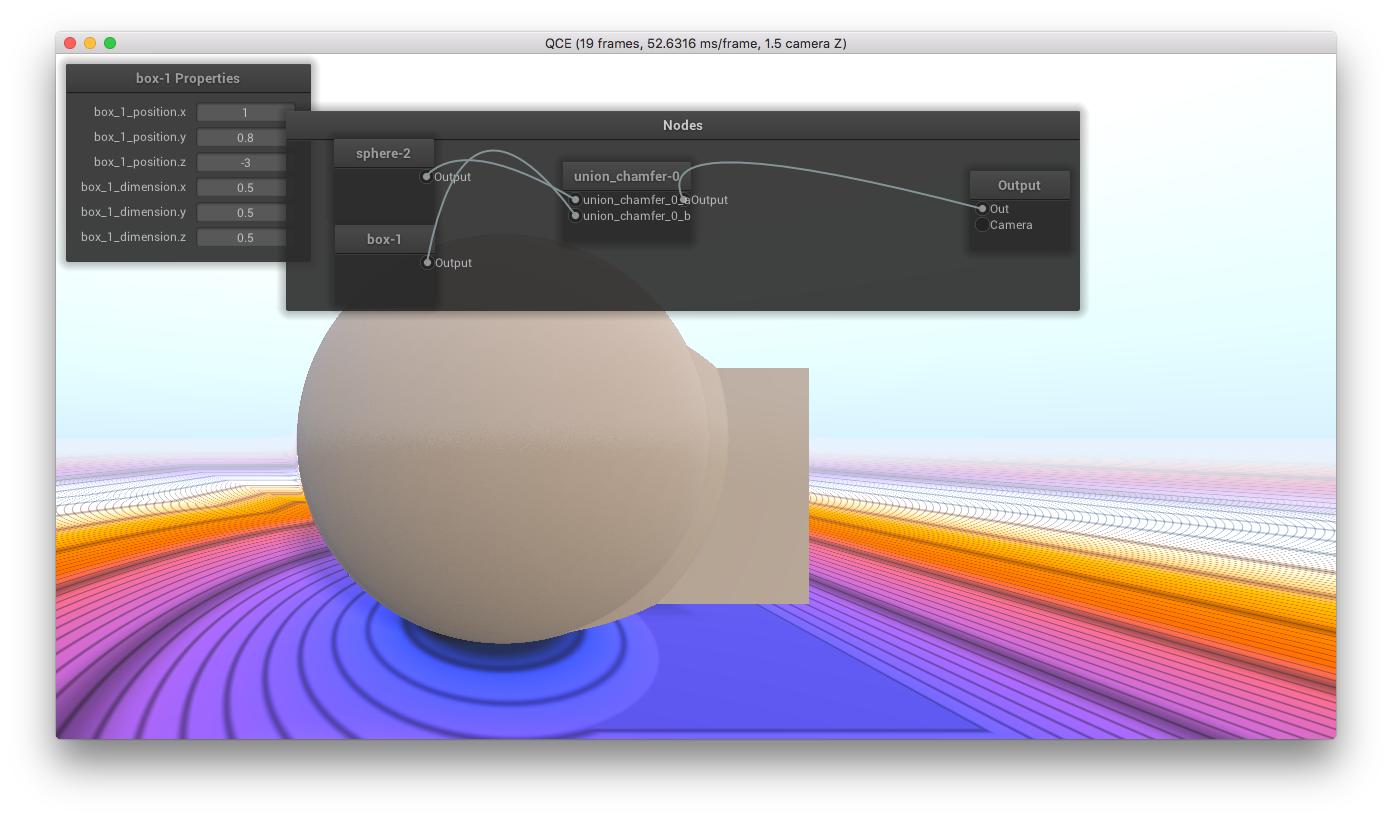
\includegraphics[width=0.9\textwidth]{img/prototype.png}
    \caption{Der Prototyp in Aktion}\label{fig:prototype:procedure}
\end{figure}
